\subsection{Задание 5. Разрешение во времени простых и сложных сигналов при
согласованной фильтрации.}

В этом задании качественно анализируется разрешение сигналов во
времени.
Качественно можно считать, что сигналы разрешены, если их максимумы
отстоят не менее, чем на величину длительности сигнала.
Требуется пронаблюдать суперпозицию двух разнесенных на величину
временной задержки сигналов на выходе согласованного фильтра. Варьируя эту
задержку, установить, какая минимальная величина задержки необходима для
успешного разрешения сигналов во времени.

\subsubsection{Прямоугольный видеоимпульс}
Проводились измерения при значениях длительности сигналов $T = 10, 20, 40$ мс. Пример суперпозиции сигналов, а также
выход с фильтра приведены на рис. \ref{fig:task5_1_10_15}.
\begin{figure}[H]
    \centering
    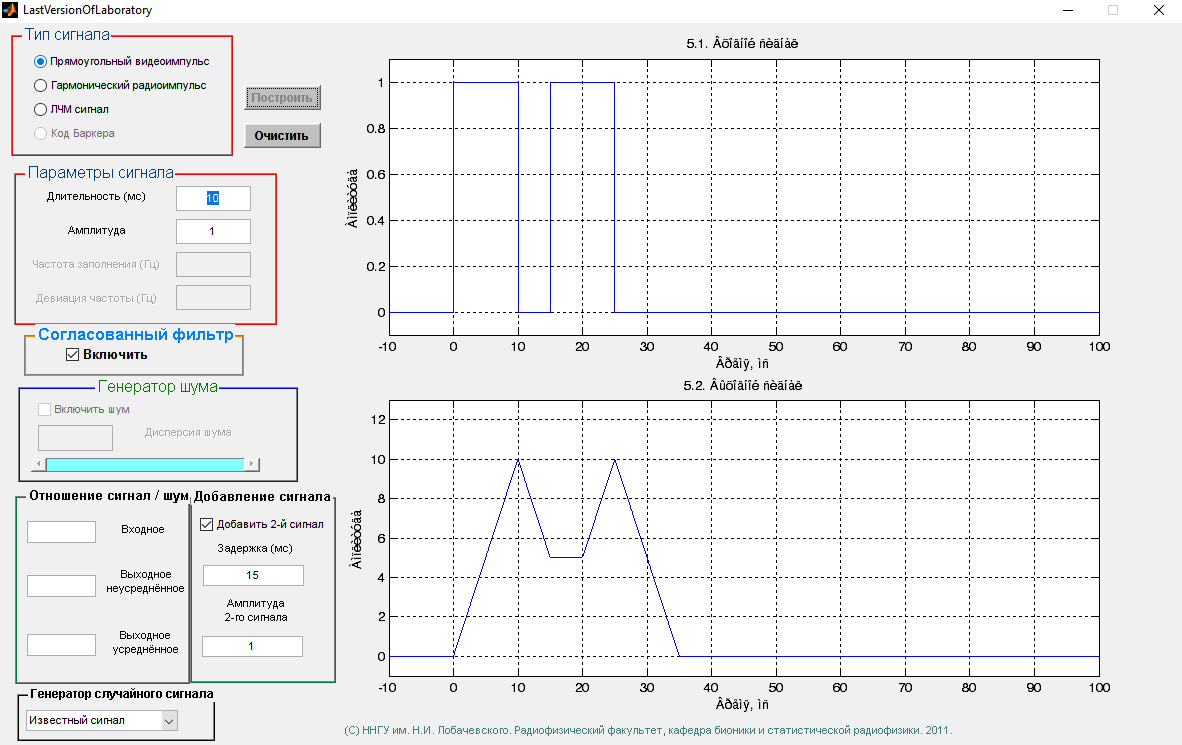
\includegraphics[width=0.9\linewidth]{imgs/task5/t5s1_dur10_del15.png}
    \caption{Прямоугольный видеоимпульс. Длительность 10 мс, задержка 15 мс}
    \label{fig:task5_1_10_15}
\end{figure}
При длительности импульса 10 мс, качественно, сигналы стали различимы при задержке в 11 мс - появились явные разделенные
пики, по которым можно различить два сигнала. Полное разделение наступило при задержке в 20 мс - т.е. удвоенной
длительности.

При увеличении длительности сигналов закономерность сохранялась - при задержке, чуть большей чем длительность сигнала,
наблюдалось выделение отдельных пиков.


\subsubsection{ЛЧМ сигнал}
Далее исследовался ЛЧМ сигнал с частотой заполнения $f=3000$ Гц, девиацией $f_\Delta = 200, 400, 800$ Гц, и
длительностью $T=10, 20, 40$ мс.
\begin{figure}[H]
    \centering
    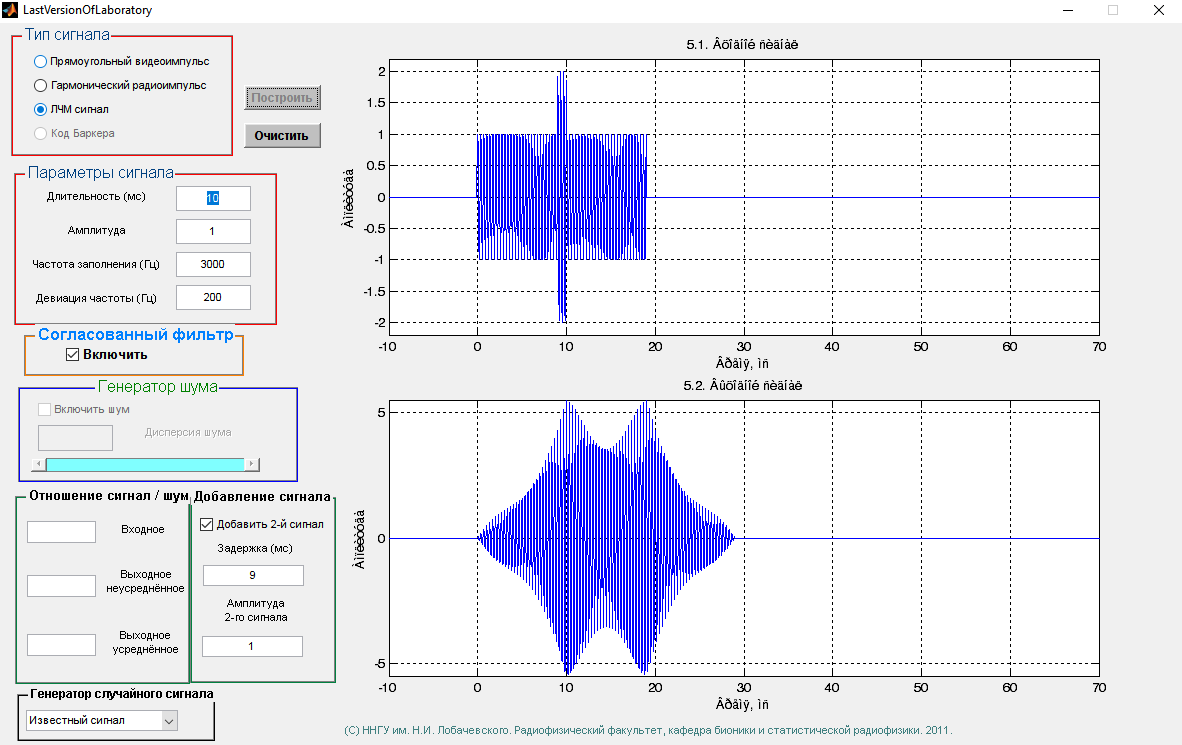
\includegraphics[width=0.9\linewidth]{imgs/task5/lfm_dev200/t5s21_dur10_del9_dev200.png}
    \caption{ЛЧМ сигнал, $T=10$ мс, $f_\Delta=200$ Гц, $t_\Delta=9$ мс}
    \label{fig:t5s21_dur10_del9_dev200}
\end{figure}
Для сигнала в $T=10$ мс, $f_\Delta=200$ Гц, значение задержки $t_\Delta$, при котором становятся различимы сигналы,
составляет $t_\Delta=6$ мс.

По результатам измерений была составлена следующая таблица, в которой указаны пороговые значения задержки в мс, при
которых сигналы становились различимыми:
\begin{table}[H]
    \begin{tabular}{|l|l|l|l|}
    \hline
    $f_\Delta$, Гц $\backslash$ T,мс   & 10 & 20 & 30 \\ \hline
    200 &  6  &  6  &  7  \\ \hline
    400 &  3  &  3.05  &  3.05  \\ \hline
    800 &  1.2  &  1.1  &  1.1  \\
    \hline 
    \end{tabular}
\end{table}
Из полученных данных видно, что увеличение длительности сигнала слабо влияет на разрешающую способность, в то время как
величина девиации, влияющая на значение базы сигнала, линейно влияет на разрешающую способность.